\section{Models for topic mining}\label{sec:models}
As seen in the related work chapter different models can be used for topic modeling in the sector of social science. In the following, the used models are presented, namely the Latent Dirichlet Allocation (LDA) model, Hierarchical Dirichlet Process (HDP) model and the Bidirectional Encoder Representations from Transformers (BERT) model, allowing to relate several topics in a mathematical context. A concise list of variables can be found in Table \ref{tab:variable_table}.

\subsection{Latent Dirichlet Allocation Model}
Latent Dirichlet Allocation (LDA), introduced by \citet{blei2003latent}, is a generative probabilistic model for data sets, specifically text. LDA aims to extract topics from the given corpus as well as new documents inexpensively.
The central thesis is that texts are represented as random mixtures of latent subjects, each of which is defined by a word distribution. This means each topic is represented by certain words which, taken together, form a subject. The text, in turn, is modeled by several subjects, each with a certain probability that models how likely the topic relates to the text.

It's critical to distinguish between LDA and traditional clustering models.
Most clustering algorithms restrict a document to a single topic, whereas LDA utilises three layers of Bayesian modeling and samples the topic node multiple times throughout a document, allowing documents to be associated with multiple themes. 

For this reason, it is a viable option for our application.
Party programs cover a wide range of topics, and the representative terms can accurately represent the content.
In Section \ref{sec:implementation}, the implementation, evaluation, and usefulness of this model will be considered. 

\subsection{Mathematical Basis}
Following the general introduction of the LDA model, we now present the mathematical context of integrating Dirichlet distributions for topic analysis. This chapter is based on \citet{newman2009distributed} and \citet{teh2006hierarchical, teh2004sharing}. In LDA the data set is given by $D$ documents which are individually integrated in the model containing $K$ not immediately recognizable topics. In this context, the data set is a vocabulary of $W$ multinomially distributed words. Integrating a statistical approach with a Bayesian formula the result is an A-Priori-distribution called the Dirichlet distribution. We define a mixing ratio $\Theta_j$ on document $j$ and a Dirichlet distribution including the parameter $\alpha$ which satisfies the concentration.
Next, it is necessary to define a probability $\Theta_{k|j}$ for the occurrence of a word $i$ in the regarded document $j$ while extracting a topic $z_{ij}=k$. The next definition we need is the probability $\Phi_{w_{ij}}$ of a word $x_{ij}$ drawn from the topic being linked to that on value w. After that we declare the word-topic distribution $\Phi_k$ as a Dirichlet distribution with parameter $\beta$ placed on it. In summary we have declared following relations for LDA:
\begin{equation}\label{eq:lda_first}
    \Theta_j\sim\mathbf{D}[\alpha] = [\Theta_{1|j},...,\Theta_{K|j}]\sim\mathbf{D[\alpha,...,\alpha]},
\end{equation}
\begin{equation}\label{eq:lda_second}
    \Phi_k\sim\mathbf{D}[\beta] = [\Phi_{1|k},...,\Phi_{W|k}]\sim\mathbf{D}[\beta,...,\beta],
\end{equation}
\begin{equation}\label{eq:lda_third}
    z_{ij}\sim\Theta_j,\ x_{ij}\sim\Phi_{z_{ij}}
\end{equation}

With \eqref{eq:lda_first}, \eqref{eq:lda_second} and \eqref{eq:lda_third} it is possible to count words belonging to a topic in one document $j$:
\begin{equation}\label{eq:lda_fourth}
    N_{kj}=\sum_{w=x_{ij}}N_{wkj},
\end{equation}
\begin{equation}\label{eq:lda_fifth}
    N_{wk}=\sum_{j}N_{wkj}
\end{equation}
The overall Dirichlet distribution with \eqref{eq:lda_fourth} and \eqref{eq:lda_fifth} is:
\footnotesize
\begin{equation}
     \begin{split}
     &p(x,z,\Theta,\Phi|\alpha,\beta)
     \sim\\
     &\prod_{j}\frac{\Gamma(K\alpha)}{\Gamma(\alpha)^K}\prod_k\Theta_{k|j}^{N_{kj+\alpha-1}}\prod_k\frac{\Gamma(W\beta)}{\Gamma(\beta)^W}\prod_w\Phi_{w|k}^{N_{wkb}+\beta-1}
     \end{split}
\end{equation}
\normalsize
% As basic assumptions for both(Variational methods & MCMC)
Having defined the Dirichlet distribution, there are two different ways for calculating posterior distribution and approximating Bayesian inference for a given word $x$. It is possibile to use variational methods like as Markov Chain Monte Carlo (MCMC) algorithms. 

$x$ is the given word and $z$ the latent topic assignment with mixing proportion $\Theta$ and topics $\Phi$ as before.
% In cite 4 (Blei) variational methods
The variational method approach from \citet{blei2003latent} first calculates the posterior distribution of hidden variables with
\begin{align}
    \begin{split}
    &p(x|\alpha,\beta)=\\
    &\frac{\Gamma(\sum_i\alpha_i)}{\prod_i\Gamma(\alpha_i)}\int_K(\prod_{i=1}^{k}\Theta_i^{\alpha_i-1})(\prod_{n=1}^N\sum_{i=1}^k\prod_{j=1}^J(\Theta_i\beta_{ij}^{x_{ij}})) d\Theta
    \end{split}
\end{align}
After this the convexity-based variational inference with Jensen's inequality omits fitting lower bounds for the logarithmic probabilities. Overall, an optimisation approach is followed during approximation with a variational parameter indexing lower bounds for yielding the tightest solution. Like in the graphical model we assume this model as tree with edges and nodes. The edges between $\Theta$, $z$ and $x$ are dropped in the next step to get a new family of distributions on the latent variables as our first variational distribution:
\begin{align}
    q(\Theta,z|\gamma,\Phi)=q(\Theta|\gamma)\prod_{n=1}^Nq(z_n|\Phi_n),
\end{align}
where $\gamma$ is placed on $\Theta$ and ($\Phi_1$,...,$\Phi_N$) is known as the multinomial parameters representing the free variational parameters. 
The optimization progress follows with Kullback-Leibler divergence between Eq. (7) and (8). The optimization problem:
\begin{align}
    \begin{split}
    &(\gamma^{*},\Phi^{*})=\\
    &arg\{min_{(\gamma,\Phi)}\{D(q(\Theta,z|\gamma,\Phi)||p(\Theta,z|x,\alpha,\beta)) \}\}
    \end{split}
\end{align}
is minimized during an iterative process for getting the derivatives. These are then set equal to zero to obtain a pair of updated equations:
\begin{align}
    \Phi_{ni}\sim\beta_{ix_n}exp\{E_q[log(\Theta_i)|\gama]\} \\
    \gamma_i=\alpha_i+\sum_{n=1}^N\Phi_{ni}
\end{align}
and compute as well the expectation within the multinomial update: 
\begin{align}
    E_q[log(\Theta_i)|\gamma]=\Psi(\gamma_i-\Psi(\sum_{j=1}^k\gamma_j)).
\end{align}
$\Psi$ can be seen as the first derivative of the logarithmic-gamma function. For a more detailed look of the calculation of the equations (9), (10), (11) and (12) have a look in the appendix in \citet{blei2003latent}. Based on the formulas above the approximation to the posterior distribution can be realized for a given data-set.
\\\\
%In tomotopy MCMC
Approximating inference with MCMC given $\Phi$ and $\Theta$ are integrated in (6) which is called collapsing. During this process the latent topics z are sampled and the current state of one variable $z_{ij}$ is omitted with following conditional probability:
\begin{align}
    p(z_{ij}=k|z^{\neg{ij}},x,\alpha,\beta)\sim\frac{N_{wk}^{\neg{ij}}+\beta}{\sum_wN_{wk}^{\neg{ij}}+W\beta}(N_{kj}^{\neg{ij}}+\alpha)
\end{align}
In general observed topics conditional probability is computed by excluding the assigned word in place \textit{$x_{ij}$} with $\neg{ij}$.
\\\\

\begin{figure}[h]
    \centering
    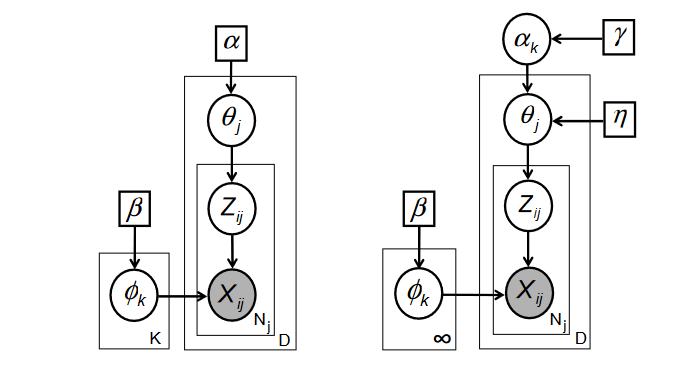
\includegraphics [width=\linewidth]{resources/LDAAndHDP.png}
    \caption{Graphical models for LDA (left) and HDP (right) \citet{newman2009distributed}}
    \label{fig:lda_hdp}
\end{figure}

\subsection{Hierarchical Dirichlet Process Model}
With the works in \citet{newman2009distributed} and \citet{teh2006hierarchical,teh2004sharing} the basic concept of HDP follows. To understand the hierarchical concept it is necessary to have an overview of basic Dirichlet Processes (DP). We define a measurable space $(\Theta, B)$ and a $\alpha_0 \in \matthbb{R}^+$. Let $G_0$ be a probability measure on $(\Theta, B)$. A arbitrary partition ($A_0,..,A_n$) of $\Theta$ with n $\in \matthbb{N}$ and n$<\infty$ the random vector included in a random probability measure G over $(\Theta, B)$ distributed with concentration parameter $\alpha_0$ is called the \textit{Dirichlet process} $DP(\alpha_0,G_0)$.
\begin{align}
    (G(A_1),...,G(A_n)) \sim Dir(\alpha_0G_0(A_1),...,\alpha_0G_0(A_n))
\end{align}
On this basis the approach of the hierarchical model combines multiple DP where a global random probability measure $G$ predetermines the basic concept of the following probability measures hierarchically structured.

Figure \ref{fig:lda_hdp} serves as a visualisation of the mathematical basis mentioned before. On this guidance the \textit{tomotopy} framework integrates both models similarly.
With right model in Figure \ref{fig:lda_hdp}, HDP, it is possible to progress by sharing clusters among related groups on multiple text documents in general.

%With the right model in Figure \ref{fig:lda_hdp}, \citet{newman2009distributed} and \citet{teh2004sharing} we clear the integration of this concept within progress other sharing cluster among related groups on multiple text documents in a general way realized in \textit{tomotopy} framework.

The general process in HDP is similar to the LDA model with simple changes. Our data set is $D$ documents with $K$ latent topics.
Here $\alpha_K$ is the $alpha$ of the global process in the highest level of the hierarchy. The Dirichlet with parameter $\alpha_{K}$ is applied on concentration $\eta$ which samples it with parameter $\frac{\eta}{K}$. Following, we omit topic mixture with parameter $\eta\alpha_K$ and word distribution like before:
\begin{align}
    \begin{split}
    &\alpha_K\sim\mathbf{D}[\gamma/K],\ \Theta_j\sim\mathbf{D}[\alpha],\ \Phi_k\sim\mathbf{D}[\beta],\\ &z_{ij}\sim\Theta_j,\ x_{ij}\sim\Phi_{z_{ij}}
    \end{split}
\end{align}
Subsequently, the direct assignment sampler for HDP is omitted for getting the posterior distribution calculated in \citet{teh2006hierarchical}. Resulting, like in LDA $\Theta$ and $\Phi$ are integrated in (6). Finally with those approaches we end up in  conditional distribution for latent topic assignments:
\begin{align}
    \begin{split}
    &p(z_{ij}=k|z^{\neg{ij}},x,\alpha,\beta,\eta)\sim\\
    &\begin{cases}\frac{N_{wk}^{\neg{ij}}+\beta}{\sum_{w}N_{wk}^{\neg{ij}}+W\beta}(N_{kj}^{\neg{ij}}+\eta\alpha_k),\ $k= prev. k$\\
    \frac{\eta\alpha_{new}}{w}, $ k=k_{new}.$\\
    \end{cases}
    \end{split}
\end{align}

\begin{table}[h]
    \begin{tabular}{|p{1cm}||p{6.5cm}| }
        \hline
        variable & description\\
        \hline
        D & number of documents\\
        W & number of different words in vocabulary\\ 
        N & number of words in data-sets\\
        K & number of topics\\
        $x_{ij}$ & $i^{th}$ investigated word in document j\\
        $z_{ij}$ & topic allocated to $w_{ij}$\\
        $N_{wk}$ & Counter: word allocated to topic\\
        $N_{kj}$ & Counter: topic allocated in document\\
        $\Phi_k$ & probability of word being suitable for topic t\\
        $\Theta_j$ & probability of topic being suitable for document j\\
        $\alpha$ & probability measure parameter placed on $\Theta_j$ \\ 
        $\beta$ & probability measure parameter placed on $\Phi_k$ \\
        $\gamma$ & concentration parameter\\
        $\eta$ & probability measure parameter applied to $\alpha_k$ placed on $\Theta_j$\\
        \hline
    \end{tabular}
    \caption{Description of used variables \citet{newman2009distributed}}
    \label{tab:variable_table}
\end{table}
% Advantage: number of topics determined by data


% tomotopy: can use adv. of multicore CPUs (with SIMD instr. set) -> faster iter. 
% Variational Bayes(VB) used in genisms LdaModel


\subsection{BERT model}
Another approach to extracting topics from party programs was using Bidirectional Encoder Representations from Transformers (BERT). 
\subsubsection{Training}
The technology of including contextual information from both, left and right side instead of only one side guarantees better results and was first introduced with the BERT model in \citet{Devlin2019BERTPO}. This behavior allows a deeper understanding of the language model.

The goal of BERT and other BERT style model's training processes is to correctly predict missing words in sentences by their context. The BERT model therefore uses two different approaches:
\begin{enumerate}
    \item Masked LM (MLM) \\
    In this approach, 15\% of the tokens are selected and these selected tokens are replaced by the following tokens as a copy of the original token sequence:
    \begin{itemize}
        \item 80\% of the tokens are replaced by [MASK] tokens
        \item 10\% of the tokens are replaced by random words
        \item 10\% of the tokens are kept the same
    \end{itemize}
    This detailed information was first published in \citet{DevlinPres}.
    The original token and modified token sequence are then embedded into vectors which are then processed by BERTs transformer encoder layers. \hyperref[sec:transformer]{Section 3.4.2} gives a more detailed view on BERT's transformer architecture. The output vectors of the classification layer are now being multiplied with the embedding matrix, allowing the model to calculate the probabilities of each word using the softmax function 
    \begin{align}
        \sigma(\textbf{z})_i = \frac{e^{z_i}}{\sum^K_{j=1} e^{z_j}}
    \end{align}
    where \textbf{z} is the input vector of \emph{K} elements and $i \in [1,K]$.
    \begin{figure}[h]
        \centering 
        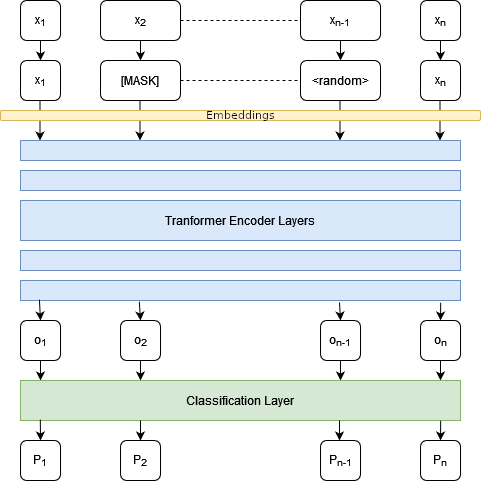
\includegraphics [width=\linewidth]{resources/BERT_MLM.png}
        \label{fig:my_label}
    \end{figure}
   
    \item Next Sentence Prediction (short NSP) \\
    Next Sentence Prediction is the process of determining whether a given sentence is the subsequent sentence to another given sentence. As an input it receives a list of pairs of two sentences of which 50\% are a combination of two subsequent sequences and the other 50\% got a random sentence as their second element without the model knowing which are which of course. The goal of the NSP model is then to identify which sentences are subsequent and which are in no positional relation. \\
    Before the input reaches the transformer model it gets preprocessed in the following steps:
    \begin{enumerate}
        \item The input is tokenized on a word basis (ex. "playing" --> ["play", "##ing"])
        \item A [CLS] token is inserted before the first sentence and a [SEP] token is inserted after each sentence.
        \item A sentence embedding layer which indicates to which sentence a token belongs.
        \item A positional embedding layer which indicates to what position a token a token belongs in the input string. This is used to represent positional relations between the input tokens.
    \end{enumerate}\\
    The sentences \emph{"my dog is cute. he likes playing"} would lead to the following output after the preprocessing steps: 
    \begin{figure}[h]
        \centering 
        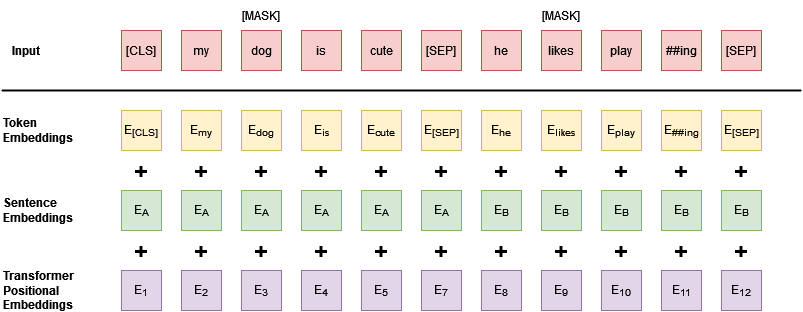
\includegraphics [width=\linewidth]{resources/NextSentence.png} \\
        \caption{\citet{Devlin2019BERTPO}. A larger version can be found in the appendix, Figure \ref{fig:next_sentence_large}.}
        \label{fig:my_label}
    \end{figure}
    \\
    The preprocessed input is then passed to the transformer model where the output is then used to calculate the probability of IsNextSequence with the softmax function.
\end{enumerate}
\subsubsection{Transformer Architecture}
\label{sec:transformer}
Transformers are the first transduction models relying entirely on self-attention mechanisms \cite{1706.03762}.
The complete architecture of one transformer is shown in Figure \ref{fig:transformer}.
\begin{figure}[h]
    \centering 
    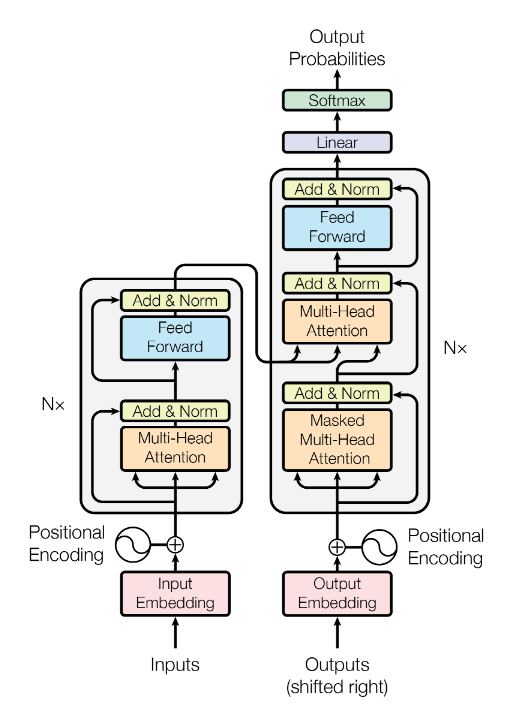
\includegraphics [width=\linewidth]{resources/Transformer} \\
    \caption{\citet{1706.03762}}
    \label{fig:transformer}
\end{figure} \\
The individual components are now being described in more detail:
\begin{itemize}
    \item \textbf{Encoder}: The encoder is shown in the left part of the figure and consists of 6 similar layers that all contain a self-attention mechanism layer and a feed-forward network layer. Every single sub-layer produces an output of dimension $d_{output} = 512$
    \item \textbf{Decoder}: The decoder (shown on the right) is pretty much similar to the encoder except for the additional maskes multi-head attention layer.
    \item \textbf{Multi-Head Attention}: The goal of an attention mechanism is to generate a weighted sum of values, where the input is a query vector and two other vectors representing key-value pairs. The multi-head attention layers are more or less the most important part of the tranformer's architecture. Their core consists of a scaled dot-product attention mechanism, which takes in three different vectors of size $d_k, d_k, d_v$, where the vector of queries and keys are of size $d_k$ and die vector of values is of size $d_v$. Since in reality the attention mechanism is applied to a set of input vectors simultaneously, the vectors are grouped in matrices. The result of the scaled dot-product attention function can then be expressed as follows: \\
    $Attention(Q, K, V) = softmax(\frac{QK^T}{\sqrt{d_k}})*V$
    \item \textbf{Feed-Forward Network}: The FFNs are basically a ReLU activation $ReLU(x) = max(0, nx)$ of a linear transition multiplied by another linear transition: \\
    $FFN(x) = max(0, xW_1+b_1)*W_2+b_2$
\end{itemize}